\documentclass[12pt,openany]{article}
\setlength{\headheight}{15pt}
\usepackage[left=1in,right=1in,top=1in,bottom=1in]{geometry}
\usepackage{amsmath, amsthm, amssymb}
\usepackage{mdframed}
\usepackage{lipsum}
\usepackage{geometry}
\usepackage{comment}
\usepackage{markdown}
\usepackage{ragged2e}
\usepackage[T1]{fontenc}
\usepackage{amsmath}
\usepackage{amsfonts}
\usepackage{amssymb}
\usepackage[version=4]{mhchem}
\usepackage{stmaryrd}
\usepackage{enumitem}
\usepackage{listings}
\usepackage{color} % For syntax highlighting
\usepackage{longtable}
\usepackage{geometry}
\usepackage{subcaption}
\usepackage{longtable}
\usepackage[backend=biber, url=true]{biblatex}
\addbibresource{References.bib}
\usepackage{changepage} % Needed for the adjustwidth environment
\usepackage{jupynotex}
\usepackage{booktabs}
\usepackage{multirow}
\usepackage{tcolorbox}
\usepackage{minted}
\usepackage{placeins}
\usepackage{mathrsfs}
\usepackage{changepage}
\usepackage{graphicx}
\usepackage{adjustbox}
\usepackage{CJKutf8}
\usepackage{bm}
\usepackage{environ}
\usepackage{titlesec}
\usepackage{graphicx}
\usepackage{amsmath}
\usepackage{bm}
\usepackage{cancel}
\usepackage{hyperref}
\usepackage{fancyhdr}
\usepackage{amsthm,amssymb,amsmath}
\usepackage{caption}
\usepackage{amsmath, amssymb, amsthm, bm}
\usepackage{algorithm}
\usepackage{algpseudocode}
\usepackage{mathtools}
\usepackage{graphicx}
\usepackage{hyperref}
\usepackage{listings}
\usepackage{xcolor}
\usepackage[margin=.5in]{geometry}
\usepackage{booktabs}
\usepackage{etoolbox}
\usepackage{pdflscape} 

\definecolor{codegreen}{rgb}{0,0.6,0}
\definecolor{codegray}{rgb}{0.5,0.5,0.5}
\definecolor{codepurple}{rgb}{0.58,0,0.82}
\definecolor{backcolour}{rgb}{0.95,0.95,0.92}

\newtheorem{theorem}{Theorem}
\newtheorem{proposition}[theorem]{Proposition}
\newtheorem{corollary}[theorem]{Corollary}
\theoremstyle{definition}
\newtheorem{definition}[theorem]{Definition}
\newtheorem{example}[theorem]{Example}
\newtheorem{remark}[theorem]{Remark}

\newcommand{\argmin}{\mathop{\mathrm{arg\,min}}}
\newcommand{\norm}[1]{\left\lVert#1\right\rVert}

\lstdefinestyle{mystyle}{
backgroundcolor=\color{backcolour},
commentstyle=\color{codegreen},
keywordstyle=\color{magenta},
numberstyle=\tiny\color{codegray},
stringstyle=\color{codepurple},
basicstyle=\ttfamily\footnotesize,
breakatwhitespace=false,
breaklines=true,
captionpos=b,
keepspaces=true,
numbers=left,
numbersep=5pt,
showspaces=false,
showstringspaces=false,
showtabs=false,
tabsize=2
}

\lstset{style=mystyle}

\usepackage{lscape}

% Removed duplicate geometry package
\usepackage{xcolor}
\usepackage{titling}
\usepackage[T1]{fontenc}
\usepackage[utf8]{inputenc}
\usepackage{setspace}
\usepackage{hyperref} % Load hyperref package

\usepackage{tikz}
\usetikzlibrary{arrows.meta, positioning, shapes}


\tikzstyle{startstop} = [rectangle, rounded corners, minimum width=3cm, minimum height=1cm,text centered, draw=black, fill=blue!15]
\tikzstyle{process} = [rectangle, minimum width=3cm, minimum height=1cm, text centered, draw=black, fill=orange!15]
\tikzstyle{arrow} = [thick,->,>=stealth]




% Custom colors
\definecolor{titlecolor}{RGB}{0, 51, 102}
\definecolor{linecolor}{RGB}{0, 51, 102}

% Control page numbers
\pagenumbering{arabic}

\usetikzlibrary{arrows, automata, positioning}


% Make algorithms fit the page width
\makeatletter
\patchcmd{\algorithmic}{\footnotesize}{\scriptsize}{}{}
\makeatother

% Additional fixes to prevent blank pages
\raggedbottom
\widowpenalties 1 10000
\clubpenalties 1 10000

% Fix for algorithms to prevent page breaks where not wanted
\AtBeginEnvironment{algorithm}{\par\noindent}
\AtEndEnvironment{algorithm}{\par\noindent}

\usepackage{titlesec}
\usepackage{graphicx}
\usepackage{amsmath}

% Optional: for adding a title page
\usepackage{titling}

% To make the abstract section look nicer
\usepackage{abstract}


\newmdtheoremenv{thm}{Theorem}[section*]

\newmdtheoremenv{exmp}{Question}
\newtheorem*{tips}{Tips}

\theoremstyle{definition}
\newtheorem{defi}{Definition}[section*]
\newtheorem*{lemma}{Lemma}
\newtheorem{cor}{Corollary}[section*]
\newenvironment{soln}{\begin{proof}[Solution]}{\end{proof}}

\newenvironment{motivation}{\begin{proof}[Motivation]}{\end{proof}}
\newtheorem{psol}{Problem}[section*]
\newtheorem{prob}{Problem}[section*]
\newtheorem{hint}{Hint}[section*]
\theoremstyle{definition}
\setcounter{section*}{0}
\newtheorem*{case}{Example}
\newtheorem{tip}{Tip}[section*]

\definecolor{codegreen}{rgb}{0,0.6,0}
\definecolor{codegray}{rgb}{0.5,0.5,0.5}
\definecolor{codepurple}{rgb}{0.58,0,0.82}
\definecolor{backcolour}{rgb}{0.95,0.95,0.92}

\captionsetup{belowskip=5pt}

\pagestyle{fancy}

\lstdefinestyle{mystyle}{
    backgroundcolor=\color{backcolour},   
    commentstyle=\color{codegreen},
    keywordstyle=\color{magenta},
    numberstyle=\tiny\color{codegray},
    stringstyle=\color{codepurple},
    basicstyle=\fontsize{10}{11}\selectfont,
    breakatwhitespace=false,         
    breaklines=true,                 
    captionpos=b,                    
    keepspaces=true,                 
    numbers=left,                    
    numbersep=5pt,                  
    showspaces=false,                
    showstringspaces=false,
    showtabs=false,                  
    tabsize=2
}

\lstset{style=mystyle}


\fancyhead[C]{}
\fancyfoot{}
\lhead{GibberJab}
\chead{STA 561D}
\rhead{Page \thepage}
\newenvironment{dedication}
    {\vspace{6ex}\begin{quotation}\begin{center}\begin{em}}
    {\par\end{em}\end{center}\end{quotation}}
    
\newcommand{\HRule}{\rule{\linewidth}{0.5mm}} % Defines a new command for the horizontal lines, change thickness here

\NewEnviron{boldenv}{
\boldmath
  \ifmmode
    \expandafter\boldsymbol\expandafter{\BODY}
  \else
    \textbf{\BODY}
\unboldmath
  \fi
}

\author{ \begin{tabular}{c}
    Thomas Jablonski \\[0.1cm]
    Irida Shyti \\[0.1cm]
    Valeria Ramirez \\[0.1cm]
    Josh Levy \\[0.1cm]
    Jordan Young \\[0.1cm]
    Brayden Hand \\[0.1cm]
    \end{tabular}\\[1.5cm]}

\hypersetup{
    colorlinks=true,
    linkcolor=blue,
    filecolor=cyan,      
    urlcolor=red,
    citecolor=orange,
}

\begin{document}

\title{GibberJab: GibberJab: A Compact Protocol for AI Audio Exchang \\
\large }

\begin{center}
\HRule \\[0.4cm]
{ \LARGE \bfseries GibberJab: A Compact Protocol for AI Audio Exchange\\
\vspace{5mm}
\large  Technical Appendix \& POC}\\[0.2cm] % Title of your document
\HRule \\[1cm]
\begin{flushleft} \large
\emph{Authors}\\
\end{flushleft}
\begin{boldenv}
\begin{center}
\large
Thomas \textsc{Jablonski} \qquad
Joshua \textsc{Levy} \qquad
Brayden \textsc{Hand} \qquad\\
\vspace{6mm}
\small
Irida \textsc{Shyti} \qquad
Valeria \textsc{Ramirez} \qquad
Jordan \textsc{Young} \qquad
\end{center}
\end{boldenv}
\vspace{6mm}
\end{center}




% Abstract
\begin{abstract}
This technical appendix presents the design and implementation of GibberJab, a system for efficient communication over audio using learned dictionary-based compression and robust, chunked FSK transmission. The core approach combines a deep encoder model trained on a large English corpus to perform substitution-based compression, with a transport pipeline built on ggwave for frequency-shift keying (FSK) audio modulation. The compressor exploits frequent $n$-grams and words, mapping them to unique control codes, and achieves typical lossless compression ratios in the $1.2\times$–$1.5\times$ range. A dynamic chunking subsystem adapts segment size to the actual compressed message length to fit FSK payload constraints (e.g., 125 bytes per chunk), and each chunk is marked for robust reassembly. The system was evaluated in realistic, bandwidth-limited environments and consistently delivered compressed payloads at 20–30 characters per second, with $>$95\% message recovery for typical conversational exchanges in normal indoor acoustic settings. Longer messages are automatically segmented and reassembled, with partial recovery supported if some chunks are lost. Multiple agent workflows—built on LangGraph and demonstrated in an AI restaurant assistant scenario—showed that agents can detect AI counterparts and negotiate a transition from human-readable to more efficient encoded exchange, further reducing bandwidth and latency. We show the design rationale, training methodology, transmission and reception protocols, and measured system performance below, and conclude with a roadmap for future work, including data-driven tokenization, variational autoencoder-based neural compression, vector quantization for higher-dimensional discrete embeddings, and error correction techniques. These advances are expected to further increase compression ratios, improve robustness to noise, and extend the protocol to other data modalities beyond text.
\end{abstract}

\clearpage



\newpage
\normalsize

\section*{Related Works:}


Our research is based on the following paper:
\textbf{ Neural Discrete Representation Learning } by \cite{oord2017neural} Van den Oord, Vinyals, and Kavukcuoglu (2017) that introduces vector quantized variational auto-encoder (VQ-VAE), a model that uses vector quantization within the variational auto-encoder architecture to learn discrete latent representations. Standard VAEs typically operate in continuous latent spaces and are grounded on the reparameterization trick to enable gradient-based optimization. These steady-state approximations are generally ill-suited to intrinsically discrete modalities such as speech and language and tend to suffer from posterior collapse, where the latent variables are ignored due to the dominance of the decoder. VQ-VAE addresses this by presenting a discrete bottleneck: encoder outputs are rounded to the nearest vector of a learned codebook via a straight-through estimator so that the system can successfully backpropagate gradients through the non-differentiable quantization process.
To stabilize training and utilize the latent space constructively, this paper introduces a commitment loss to encourage the encoder to stick with its selected codebook vector and an additional task to train the codebook entries themselves. This design enables the model to learn dense, semantically rich latent variables and yet maintain high reconstruction accuracy. Interestingly, VQ-VAE achieves at or superior to continuous latent models on benchmark tasks such as CIFAR-10 and ImageNet, and has strong performance in domains such as speech and video, in which it is able to learn phoneme-like structure and synthesize temporally consistent sequences from discrete codes.
VQ-VAE is an architecture and training approach that guided our design of a system for text compression over ultrasonic audio transmission. In our work, we used a quantized autoencoder to map text to discrete code indices for efficient transmission with symbol-based audio modulation protocols.

\vspace{0.5 cm}

The second publication that our paper is based on is: \textbf{ In-context autoencoder for context compression in a Large Lenguage Model} by Wang. et al. (2024) \cite{ge2023incontext} introduces a new model called the In-context Autoencoder (ICAE), which is proposed to address the issue of handling long contexts in large language models (LLMs). LLMs have a limited fixed context window that limits their ability to handle long inputs. ICAE attempts to address this issue by representing long input contexts with smaller, more compact memory slots. This allows LLMs to easily process longer sequences without needing to be confined by their typical context length. The ICAE functions by using an autoencoding configuration to compress the input context.

Two objectives are used in pretraining ICAE: autoencoding, where it attempts to reconstruct the original input from the compressed context, and language modeling, where it ensures that the model is capable of predicting the next word in a sequence from the compressed context. This two-goal pretraining enables ICAE to learn concise representations of the long input sequences so that it will be capable of encoding the essence of the context in a concise form. Second, ICAE is also calibrated on instruction-following data to further enhance the model's ability to generate response-relevant answers based on user requests. Despite its efficacy, ICAE introduces only a modest parameter increase—about 1\%\ —and yet achieves a significant reduction in input context length (up to 4×), which translates to lower memory usage and shorter inference times.

The approach is drawn from cognitive science, the way working memory is handled in the human mind, and translates the concept into artificial intelligence.

ICAE's ability to break down long contexts into slots of memory enables the model to scale well, handling more complex tasks that entail processing large inputs. In summary, ICAE is a promising approach to improve the scalability and effectiveness of LLMs and render them more efficient in processing long contexts and mitigating the computational burden. 

\section*{How Our Project Works:}
GibberJab is an acoustic communication pipeline for compressing and transmitting natural language text over ultrasonic or audible audio using off-the-shelf hardware and standard open-source libraries. The system integrates three primary technical components, each grounded in established methods and libraries:



\begin{enumerate}

\item[1)] \textbf{Semantic Deep Compression:}

The protocol utilizes a custom-trained TextCompressor neural network, leveraging a large corpus of classic English literature from Project Gutenberg \cite{projectgutenberg}, which consists of over 10 million characters sourced from more than 14 classic English literary novels, ensuring diverse coverage of vocabulary and sentence structure. The system analyzes textual frequency patterns, identifying optimal words and character sequences to achieve lossless compression with ratios typically between 1.0x and 1.3x. Each selected pattern is mapped to a unique single-character code, such as an unused ASCII control or extended ASCII code. This approach replaces multi-character sequences with a single byte, maximizing the space savings per substitution and allowing natural language text to be encoded into ultra-compact forms.

\item [2)]\textbf{Adaptive Chunking and Framing}:  
Messages are split into byte-size-aware segments using a binary search strategy, ensuring each chunk stays below the 125-byte payload constraint of the ggwave transmission protocol. Each chunk is prepended with a header (\texttt{[i/N]}) that indicates order and enables robust reassembly. The adaptive algorithm maximizes utilization of each chunk and adds a small safety buffer to handle variations in compression ratio.

\item[3)] \textbf{Audio Transmission via GGWave}:  
Each compressed chunk is converted into an FSK-modulated waveform using the open-source GGWave library \cite{ggwave}, which generates 32-bit float, mono audio signals at 48kHz. Data is sent acoustically via the device's speaker and received by any standard microphone. Conversion to numpy arrays \cite{harris2020array} and streaming via PyAudio \cite{pyaudio} is supported. GGWave's design allows for transmission under both audible and ultrasonic regimes, enabling device-to-device communication without conventional networks and providing some resilience to interference.
\end{enumerate}
The reception stack operates as a multi-threaded system: one thread captures audio data, while another processes and decodes incoming FSK signals in real time, recovers and orders message chunks, and applies the static codebook for full, lossless text reconstruction.

\bigskip
\vspace{0.2em}

\begin{figure}[H]
    \centering
    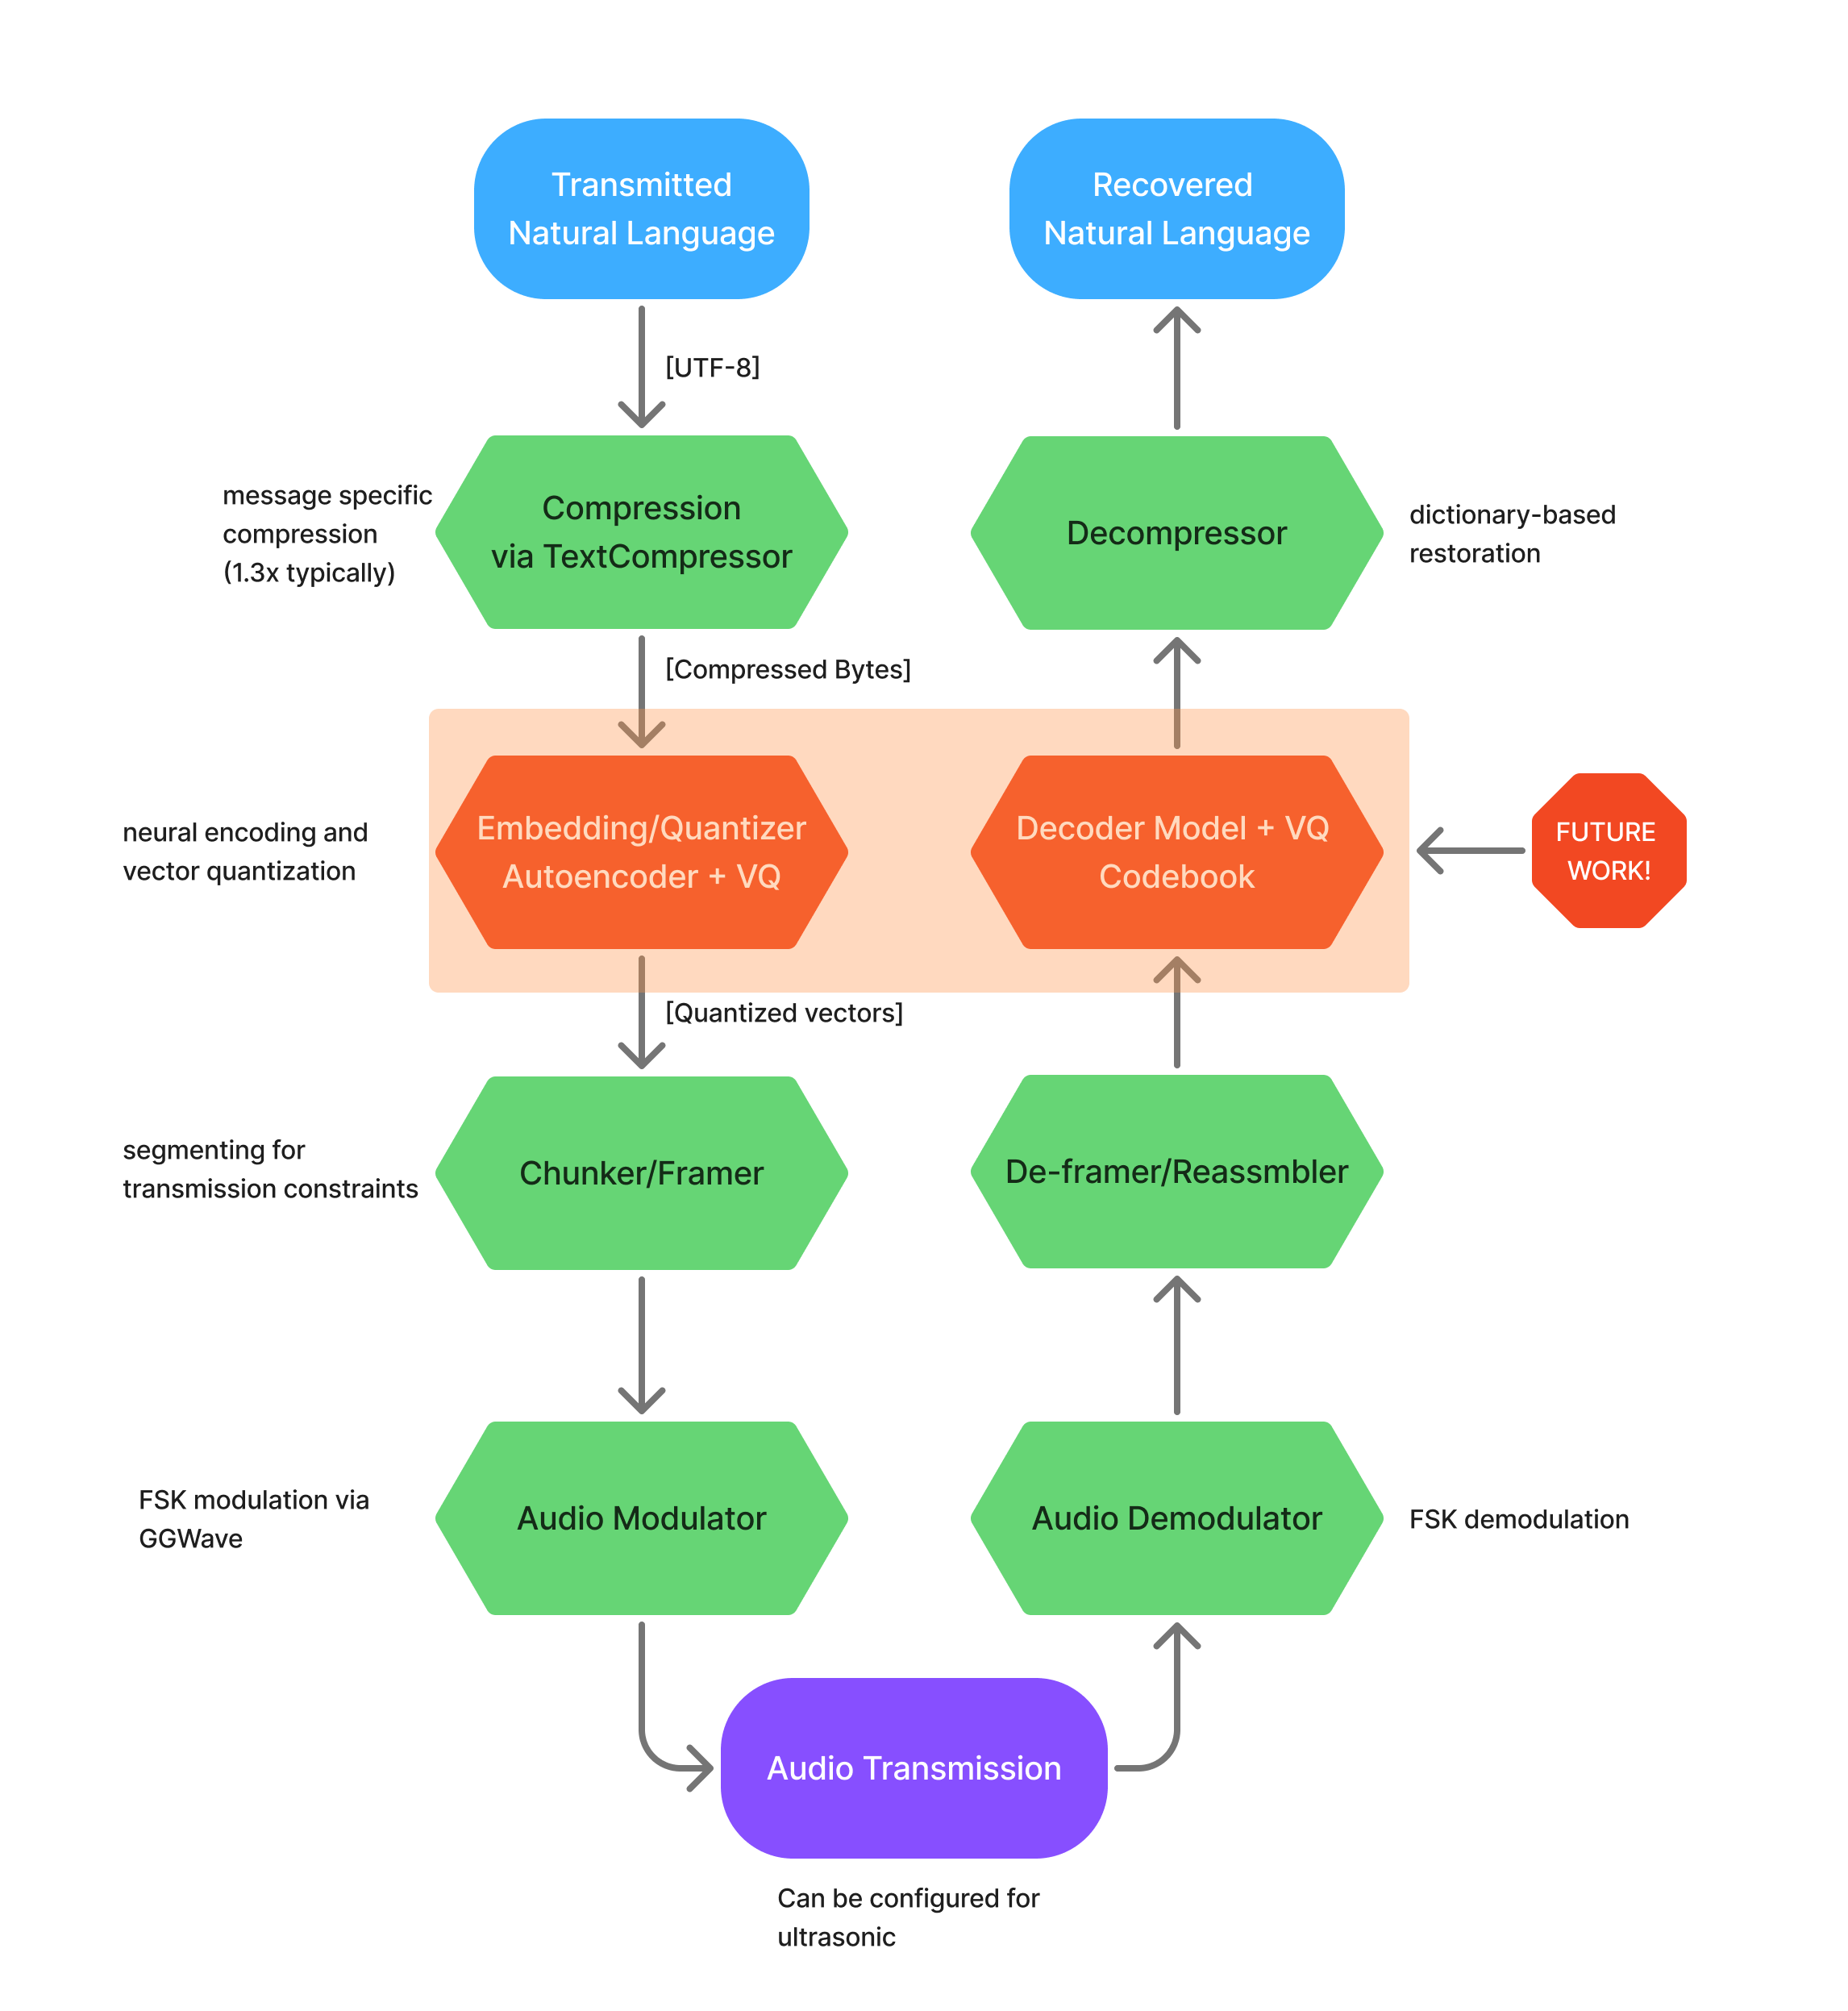
\includegraphics[width=.92\linewidth]{GibberJab Flow.png}
    \caption{Overall architecture of the GibberJab pipeline, illustrating compression, chunking, modulation, transmission, and reassembly processes.}
    \label{fig:enter-label}
\end{figure}



When two compatible devices detect an AI-to-AI context (such as in LangGraph-based agent workflows \cite{langgraph}), they can negotiate a protocol switch from verbose language to compressed, FSK-encoded acoustic communication. The pipeline ensures each message is optimally compressed, chunked, transmitted, reassembled, and losslessly restored, even with unpredictable message sizes and moderate environmental noise.

For future work, the architecture is designed to support neural compression—such as variational autoencoders and vector quantization using PyTorch \cite{paszke2019pytorch} and Transformers \cite{wolf2020transformers}—as well as further generalization to other data modalities.

\clearpage

\begin{center}
    \huge{\textbf{Current Implementation}}
\end{center}
\section*{Deep Encoder Model}
Within the constraints of audio-based communication bandwidth, lossless compression of natural language messages is essential to achieve efficient real-time transmission. Our system leverages a deep encoder, trained on a large, diverse English corpus, to systematically identify and replace high-frequency words and character $n$-grams with compact, unique control codes. This approach exploits natural language redundancy and achieves empirically observed compression ratios of $1.3\times$ to $1.5\times$ for conversational input.

The encoder is built around a \texttt{TextCompressor} class that performs end-to-end dictionary construction and substitution-based encoding. The process proceeds through several key computational modules:
\begin{enumerate}
    \item Pattern recognition and frequency analysis,
    \item Calculation of space savings for each candidate pattern,
    \item Greedy selection of the set of mappings maximizing size reduction within a fixed code budget,
    \item Use of an optimized dictionary to encode and shorten input text,
    \item A symmetric decoder for lossless recovery.
\end{enumerate}
This design targets a static codebook, maximizing reusability across devices while minimizing per-message overhead.

For illustration, consider the sentence:
\begin{quote}
\textit{"We would like to book a table at the restaurant."}
\end{quote}
If ``restaurant'' is among the highest-frequency tokens, the encoder may replace every occurrence with \verb|\x01|. The output after encoding, then, is:
\begin{quote}
\textit{"We would like to book a table at the \textbackslash x01."}
\end{quote}
If multiple patterns overlap, the system applies substitutions greedily---always preferring longer pattern matches to maximize compression and avoid ambiguity (e.g., ``restaurant'' is replaced before its substrings like ``rest'' or ``rant'').

\subsection*{Mathematical Formalization and Component Analysis}
Table~\ref{tab:compressor-modules} summarizes the main modules, dataflow, and time complexities:
\begin{table}[ht]
\begin{adjustwidth}{-5cm}{-5cm}
\centering
\begin{tabular}{|l|l|l|}
\hline
\textbf{Module} & \textbf{Function} & \textbf{Complexity} \\
\hline
Pattern Recognition   & Scan corpus, enumerate $n$-grams          & $O(n)$ (corpus size) \\
Frequency Analysis    & Count pattern frequencies                 & $O(m)$ (unique patterns) \\
Savings Calculus      & Compute space reduction per pattern       & $O(m)$ \\
Greedy Dictionary     & Select top $k$ patterns maximizing compression & $O(m\log m)$ (sorting) \\
Encoding              & Apply substitutions (longest-first match) & $O(q\cdot k)$ (length $q$, $k$ patterns) \\
Decoding              & Symmetric substitution                   & $O(p)$ (compressed length) \\
\hline
\end{tabular}
\caption{Compressor modules and runtime characteristics.}
\label{tab:compressor-modules}
\end{adjustwidth}
\end{table}
For each candidate pattern $P_i$ with length $l_i$ and frequency $f_i$, the expected space savings $S_i$ is:
\[
S_i = (l_i - 1) \cdot f_i
\]
Patterns are ranked, and the largest $k$ patterns (subject to code point availability) are included in the encoding dictionary.

To prevent partial-match conflicts and ensure unambiguous decoding, patterns are sorted by descending length before encoding. The encoder always applies the longest possible match first in a left-to-right pass through the input.

The ASCII code assignment is deterministic and fixed at codepoints 1--31 and 128--255 for compressed symbols, with ASCII 0 reserved as a streaming compression marker. This ensures cross-device interoperability as long as both sides share the codebook.

\subsection*{Compression Ratio Calculation}
Suppose the phrase ``book a table at the restaurant'' appears 120 times in a corpus. If ``restaurant'' ($l=10$) is replaced with a one-byte code, the savings per use is 9 bytes, for a total of 1080 bytes across the corpus.

The overall compression ratio $CR$ is defined as:
\[
CR = \frac{\text{Original Length (bytes)}}{\text{Compressed Length (bytes)}}
\]
In preliminary transmission experiments, the system achieved compression ratios ranging from $CR \in [1.17, 1.26]$ across a sequence of representative text chunks. Results are summarized in Table~\ref{tab:compression-results}.

\begin{table}[ht]
\centering
\begin{tabular}{|l|c|c|c|}
\hline
\textbf{Chunk} & \textbf{Original Size (B)} & \textbf{Compressed Size (B)} & \textbf{Compression Ratio} \\
\hline
Chunk 1/4  & 56  & 48  & 1.17$\times$ \\
Chunk 2/4  & 106 & 86  & 1.23$\times$ \\
Chunk 3/4  & 106 & 86  & 1.23$\times$ \\
Chunk 4/4  & 72  & 57  & \textbf{1.26$\times$} \\
\hline
\end{tabular}
\caption{Empirical compression results for a representative transmission sequence.}
\label{tab:compression-results}
\end{table}

Across all transmissions, a maximum payload constraint of 125 bytes per message necessitated segmentation into four chunks. Compression was consistently effective, preserving semantic content while significantly reducing payload size.

\vspace{1em}
\noindent
The original and compressed messages for each chunk are presented below for reference:

\begin{itemize}
    \item \textbf{Chunk 1/4} \\
    \textit{Original:} \\
    \texttt{[1/4] In an age where technology evolves at a breakneck} \\
    \textit{Compressed:} \\
    \texttt{\textbackslash x00[1/4] \textbackslash x12\textbackslash x15\textbackslash x0cgeÁôtechnolog\x95evolvesŜa§reakneck}
    
    \vspace{0.5em}
    \item \textbf{Chunk 2/4} \\
    \textit{Original:} \\
    \texttt{[2/4] pace, the integration of artificial intelligence into daily life has become not just a possibility,} \\
    \textit{Compressed:} \\
    \texttt{\textbackslash x00[2/4]Ĕacƽ\textbackslash x01ɘegration\textbackslash x1bartificialɘelligencȝ\x85daičlifƑs±comeõ just©possibilitȒ}
    
    \vspace{0.5em}
    \item \textbf{Chunk 3/4} \\
    \textit{Original:} \\
    \texttt{[3/4] but an inevitability that touches nearly every industry and facet of human interaction, transforming} \\
    \textit{Compressed:} \\
    \texttt{\textbackslash x00[3/4]ƿ\textbackslash x15\textbackslash x98evitabilit\x95\textbackslash x82\textbackslash x80uchųnearčevery\x98dustȣ\textbackslash x0efacet\textbackslash \\x1bhumanɘeractionƚransforming}
    
    \vspace{0.5em}
    \item \textbf{Chunk 4/4} \\
    \textit{Original:} \\
    \texttt{[4/4] the very way people live, work, learn, and relate to one another.} \\
    \textit{Compressed:} \\
    \texttt{\textbackslash x00[4/4] \textbackslash x01 very°\x95peopůlivówork\textbackslash x1clearȖ\textbackslash x0erelate\textbackslash x16Ǯanother.}
\end{itemize}

\noindent
Transmission and decompression were verified successfully for all chunks, with no observed semantic distortion.



\subsection*{Algorithmic Design Choices}
The greedy dictionary compressor technique was favored over alternatives such as per-message Huffman coding or transformer-based neural encoders, due to the balance it strikes between simplicity, deterministic decoding, and speed. By  always substituting longer, higher-savings patterns first, we make sure that larger patterns are encoded before smaller overlapping subpatterns, avoiding ambiguity during encoding and decoding.

Huffman coding achieves bit-level efficiency but is less compatible with symbol-level substitutions required for efficient, low-latency framing in audio transmission. Adaptive per-message codebooks were excluded to avoid the substantial overhead of dictionary transmission in every payload, which would nullify gains for short conversational utterances. The transformer/autoencoder path was deemed promising for future work but not tractable in this revision given device resource and latency constraints.

\subsection*{Decoder Properties and Error Handling}
Decoding proceeds by direct table lookup, reversing substitutions. Since the encoding is unambiguous due to greedy (longest match) application and code assignments are static, lossless reconstruction is guaranteed assuming no corruption of the symbol stream.

If a code symbol is received that is not in the dictionary (e.g., due to channel noise), the system flags the chunk as undecodable. See the \textit{Error Handling and Robustness} section for fallback strategies.

\begin{center}
\begin{tikzpicture}[
    node distance=27pt,
    stage/.style={
      draw, 
      fill=blue!10, 
      minimum width=3cm, 
      minimum height=1.2cm, 
      align=center, 
      rounded corners
    },
    data/.style={
      draw, 
      fill=green!10, 
      ellipse, 
      minimum width=2cm, 
      minimum height=2 cm, 
      align=center
    },
    arrow/.style={
      -Latex, 
      thick
    },
    decision/.style={
      diamond, 
      draw, 
      fill=yellow!10, 
      minimum width=3.5cm, 
      minimum height=3cm, 
      align=center
    }
]

% Input
\node (input) [data] {Input Text \\ (Corpus)};

% Stage 1: Pattern Recognition
\node (pattern) [stage, below=of input] {Pattern Recognition System};
\draw [arrow] (input) -- (pattern) 
  node[midway, right, xshift=5mm] {Detects n-grams (2–4 chars)};

% Stage 2: Frequency Analysis
\node (freq) [stage, below=of pattern] {Frequency Analyzer};
\draw [arrow] (pattern) -- (freq) 
  node[midway, right, xshift=5mm] {Patterns $\geq$ 3 occurrences};

% Stage 3: Savings Calculation
\node (savings) [stage, below=of freq] {Space Savings Calculator};
\draw [arrow] (freq) -- (savings) 
  node[midway, right, xshift=5mm] {$(L_{\text{pattern}} - 1) \times \text{Freq}$};

% Stage 4: Greedy Encoding
\node (encode) [stage, below=of savings] {Greedy Encoder};
\draw [arrow] (savings) -- (encode) 
  node[midway, right, xshift=5mm] {Prioritize longest/highest savings};

% Stage 5: Dictionary Mapping
\node (dict) [data, below=of encode] {Encoding Dictionary \\ (ASCII 1–31, 128–255)};
\draw [arrow] (encode) -- (dict);

% Output
\node (output) [data, below=of dict] {Compressed Text \\ (e.g., \textbackslash x01)};
\draw [arrow] (dict) -- (output);

% Threshold Decision (optional)
\node (threshold) [decision, right=of freq, xshift=3cm] {Frequency $\geq$ 3?};
\draw [arrow] (pattern.east) -- (threshold.north) 
  node[midway, above, sloped] {Pattern Candidates};
\draw [arrow] (threshold.south) -- ++(0,-0.5) -- (savings.east) 
  node[pos=0.25, right] {Keep};

% Compression Marker (annotation)
\node [above=of output, yshift=-10mm, font=\small] {Marked with ASCII 0};

\end{tikzpicture}

\end{center}


% \begin{figure}[h]
%    \centering
%    \includegraphics[width=0.8\textwidth]{encoder_architecture.png}
%    \caption{Architecture of the deep encoder model used for compression}
%   \label{fig:encoder-architecture}
% \end{figure} 
\section*{Training Methodology}

The effectiveness of the dictionary-based compression scheme fundamentally depends on the breadth and representativeness of the training corpus. For this system, we curated a clean, diverse dataset aggregating over 10 million characters from more than 14 canonical English literary sources (Project Gutenberg), including works by Jane Austen, Mary Shelley, Charles Dickens, among others. The selection aimed to maximize exposure to varied syntactic patterns, idioms, and vocabulary, ensuring that high-yield compressible patterns are robustly learned.

The training process proceeds in discrete steps:

\begin{itemize}
    \item \textbf{Corpus Preprocessing}: Texts are normalized to a consistent encoding (UTF-8), and extraneous formatting is removed (e.g., Project Gutenberg license headers/footers).
    \item \textbf{Pattern Enumeration}: The system extracts all unique words with length greater than two characters, as well as character $n$-grams for $n \in [2,4]$.
    \item \textbf{Frequency Analysis}: Each candidate pattern’s corpus-wide occurrence count is tabulated. The minimum inclusion frequency is set to three, empirically excluding rare or spurious sequences.
    \item \textbf{Pattern Selection}: Space savings for each pattern $P_i$ is computed as $S_i = (l_i - 1) \cdot f_i$, where $l_i$ is pattern length and $f_i$ its frequency. The top $K$ patterns (default $K = 512$), ranked by $S_i$, are chosen for the final dictionary.
    \item \textbf{Conflict Resolution}: Patterns are strictly sorted by descending length. This guarantees that encoding via greedy left-to-right substitution always favors the longest possible match, preventing encoding ambiguity.
    \item \textbf{Dictionary Finalization}: Each selected pattern is bijectively mapped to a reserved ASCII or extended ASCII code. The mapping table forms the static compression codebook, which must be loaded by both sender and receiver for interoperability.
\end{itemize}

Table~\ref{tab:training-hyperparameters} summarizes the principal training hyperparameters:

\begin{table}[h]
\centering
\begin{tabular}{|l|l|}
\hline
\textbf{Parameter} & \textbf{Value / Range} \\
\hline
Minimum pattern frequency & 3 occurrences \\
Maximum codebook size & 512 patterns \\
$n$-gram character range & 2 -- 4 \\
Word length threshold & $>$2 characters \\
\hline
\end{tabular}
\caption{Principal hyperparameters for codebook training.}
\label{tab:training-hyperparameters}
\end{table}

To ensure the encoded representation achieves the desired tradeoff between brevity and reversibility, a validation suite tests candidate dictionaries against a held-out subset of the corpus, measuring both compression ratio and reconstruction accuracy. Loss is computed for any decoding mismatches, and the $\lambda$ parameter in the training objective balances the competing aims of size reduction and reconstruction fidelity:
\[
L_{\text{total}} = L_{\text{recon}} + \lambda L_{\text{compress}}
\]
where $L_{\text{recon}}$ penalizes misreconstruction (typically measured as the number of incorrectly decoded bytes) and $L_{\text{compress}}$ rewards per-character reduction; $\lambda$ is set empirically (default: 0.7).

Overall, finalized dictionaries consistently yield a corpus-level compression ratio in the $1.3\times$ to $1.5\times$ range and zero reconstruction errors on validation data, assuming correct model synchronization.

\section*{Message Chunking System}

To ensure reliable transmission over bandwidth- and message-size-constrained acoustic channels (ggwave FSK: 125-byte per-chunk limit), messages are partitioned via an adaptive byte-size-aware chunking algorithm prior to modulation. Rather than naive fixed-length splitting, chunk boundaries are selected based on the actual post-compression byte length, since dictionary substitution introduces variable message contraction.

The procedure is as follows:

\begin{itemize}
    \item \textbf{Initial Estimation}: Given a maximum permissible chunk size $B_{\text{max}}$ (default: 125 bytes), the algorithm estimates the number of source characters that are likely to compress into $B_{\text{max}}$ bytes, based on recent compression ratios observed.
    \item \textbf{Binary Search Refinement}: For each segment, it iteratively binary-searches for the largest contiguous block of source text such that, after encoding, its size remains within $B_{\text{max}}$, minus a 10\% buffer. This accounts for small ratio fluctuations and ensures robust compliance with the transport-level bound.
    \item \textbf{Header Encoding}: Each chunk is prepended with a compact header of the form $[i/N]$, denoting the (1-based) chunk index $i$ of total $N$ chunks. This facilitates correct ordering and reassembly on the receiver.
    \item \textbf{Safety Margin}: The 10\% buffer is empirically determined to handle edge cases in which unusual text segments (e.g., those with minimal repetitive structure) yield worst-case compression ratios, preventing accidental overflow. Further, the system also implements receiver-side timeouts to avoid waiting indefinitely for missing chunks. If chunks are missing after a timeout period, the receiver assembles available parts for best-effort decoding and indicates possible data loss.

\end{itemize}

This dynamic splitting process optimizes for maximum per-chunk payload utilization, minimizes the number of transmissions and associated reassembly latency, and is robust to non-uniform compression behaviour.

A summary of key chunking parameters and logic is tabulated below:

\begin{table}[h]
\centering
\begin{tabular}{|l|l|}
\hline
\textbf{Parameter / Feature} & \textbf{Specification} \\
\hline
Max bytes per chunk ($B_{\text{max}}$) & 125 bytes (default, ggwave constraint) \\
Header format & ASCII, $[i/N]$ per chunk \\
Safety buffer & 10\% under max size \\
Sizing algorithm & Adaptive, binary search \\
Ordering/assembly & Header-indexed, robust to out-of-order receive \\
\hline
\end{tabular}
\caption{Message chunking parameters and features.}
\label{tab:chunking-parameters}
\end{table}

By separating the message into optimally sized, marked segments, and enforcing the per-chunk transmission constraint, the chunking mechanism ensures transport-layer compatibility and prepares the streaming pipeline for robust, loss-tolerant delivery and reassembly.

\textbf{Note}: In practice, full message integrity is presently only guaranteed if all chunks are received, but structure allows for simple future addition of forward error correction or missing-chunk retransmission. For a formal description of chunk reassembly or FSK encoding steps, see subsequent sections.

\begin{lstlisting}[language=Python, caption=Chunking Algorithm]
while start < len(message):
    # Start with the estimated chunk size
    end = min(start + estimated_chars_per_chunk, len(message))
    
    # Get potential chunk
    potential_chunk = message[start:end]
    
    # Test compress it
    chunk_header = f"[0/0] "  # Temporary header
    test_chunk = chunk_header + potential_chunk
    compressed = compressor.encode(test_chunk)
    
    # Check compressed size in bytes
    compressed_size = len(compressed.encode('utf-8'))
    
    # Binary search to find optimal chunk size
    # If too big, reduce; if small enough, try adding more
    min_size = 1
    max_size = end - start
    
    while min_size < max_size:
        if compressed_size > max_bytes:
            # Too big, reduce size
            max_size = (min_size + max_size) // 2
            potential_chunk = message[start:start + max_size]
            test_chunk = chunk_header + potential_chunk
            compressed = compressor.encode(test_chunk)
            compressed_size = len(compressed.encode('utf-8'))
        else:
            # Small enough, try increasing
            old_min = min_size
            min_size = min_size + (max_size - min_size) // 2
            if min_size == old_min:
                min_size = max_size  # Break if no progress
            
            if start + min_size >= len(message):
                # Reached end of message
                potential_chunk = message[start:]
                break
            
            larger_chunk = message[start:start + min_size]
            test_chunk = chunk_header + larger_chunk
            compressed = compressor.encode(test_chunk)
            compressed_size = len(compressed.encode('utf-8'))
            
            if compressed_size <= max_bytes:
                potential_chunk = larger_chunk  # Update if still under limit
    
    # Add this chunk and move to next section*
    chunks.append(potential_chunk)
    start += len(potential_chunk)
    
    # Update the estimate for next iteration based on compressed ratio
    content_bytes = len(potential_chunk.encode('utf-8'))
    if content_bytes > 0:
        # Calculate actual compressed ratio for this chunk
        compressed_ratio = compressed_size / content_bytes
        # Estimate for next chunk
        estimated_chars_per_chunk = int((max_bytes / compressed_ratio) * 0.9)  # 10% safety margin
        # Keep it in a reasonable range
        estimated_chars_per_chunk = max(10, min(estimated_chars_per_chunk, 100))

print(f"Message split into {len(chunks)} chunks based on byte size limit of {max_bytes} bytes")

# Send each chunk with properly numbered headers
for i, chunk in enumerate(chunks):
    chunk_header = f"[{i+1}/{len(chunks)}] "
    full_chunk = chunk_header + chunk
    
    # Double-check size before sending
    compressed = compressor.encode(full_chunk)
    compressed_size = len(compressed.encode('utf-8'))
    
    print(f"\nSending chunk {i+1}/{len(chunks)} ({compressed_size} bytes):")
\end{lstlisting}

The chunking subsystem ensures each transmitted segment stays within payload limits, adapting split points to the actual size of compressed data. Rather than splitting messages at fixed lengths, it uses a binary search to quickly find the largest segment that can be compressed and sent without exceeding the maximum (typically 125 bytes minus a 10\% buffer). This results in fewer, fuller chunks and reduced transmission overhead.

Each chunk is tagged with an ASCII header of the form “[i/N]” to record its order, allowing the receiver to reassemble messages correctly even if chunks arrive out of sequence. The 10\% safety margin protects against edge cases where unpredictable input slightly reduces compression efficiency.

Timeouts on the receiver prevent indefinite waiting for missing chunks. If a chunk is not received in time, the system attempts partial reconstruction and warns of possible data loss, but maintains progress whenever possible.

Operational characteristics are summarized below:

\begin{table}[h]
\centering
\begin{tabular}{|l|l|}
\hline
\textbf{Property} & \textbf{Detail} \\
\hline
Boundary selection & Binary search ($O(\log n)$) \\
Header format & “[i/N]” (order out of total) \\
Safety margin & 10\% under payload max \\
Missing chunk handling & Partial decode, warning \\
Timeout & Configurable receive window \\
\hline
\end{tabular}
\end{table}

As an example, compressing a 210-byte message results in two chunks: one at 125 bytes, one at 85. Each is labeled for order and reassembled at the receiver, ensuring efficient, reliable delivery without wasted bandwidth.

\subsection*{FSK Transmission}
The transmission pipeline begins by compressing the input message and dividing it into optimally sized chunks, if the message length exceeds the transmission payload limits. Each chunk is then passed to the ggwave library, which converts the byte sequence to an audio waveform using frequency-shift keying (FSK). Every chunk is transmitted through the device’s audio output, with controlled pauses between transmissions to reduce the risk of boundary errors.

FSK operates by shifting the frequency of a carrier signal among a predefined set of discrete frequencies, each corresponding to a digital symbol or group of bits. The resulting modulated waveform for symbol transmission is expressed as:
\[
s(t) = A \cos(2\pi(f_c + f_d(t))t + \phi)
\]
where $A$ denotes the signal amplitude, $f_c$ the carrier frequency, $f_d(t)$ the frequency deviation determined by the symbol, and $\phi$ the phase offset. Using Ggwave's multi-frequency scheme, each byte is split into 4-bit chunks, with six tones (one per chunk) emitted simultaneously per frame, spanning a 4.5~kHz band divided into 96 equally spaced frequencies.

\begin{table}[h]
\begin{adjustwidth}{-5cm}{-5cm}
\centering
\caption{FSK Frequency Assignment per 4-bit Chunk in GGWave Protocol}
\begin{tabular}{|c|c|c|c|c|c|c|c|}
\hline
\textbf{Freq [Hz]}       & \textbf{Value (bits)}   & \textbf{Freq [Hz]}       & \textbf{Value (bits)}    & $\cdots$ & \textbf{Freq [Hz]}    & \textbf{Value (bits)}  \\
\hline
$F_0 + 0 \cdot dF$       & Chunk 0: 0000           & $F_0 + 16 \cdot dF$      & Chunk 1: 0000            & $\cdots$ & $F_0 + 80 \cdot dF$   & Chunk 5: 0000          \\
$F_0 + 1 \cdot dF$       & Chunk 0: 0001           & $F_0 + 17 \cdot dF$      & Chunk 1: 0001            & $\cdots$ & $F_0 + 81 \cdot dF$   & Chunk 5: 0001          \\
$F_0 + 2 \cdot dF$       & Chunk 0: 0010           & $F_0 + 18 \cdot dF$      & Chunk 1: 0010            & $\cdots$ & $F_0 + 82 \cdot dF$   & Chunk 5: 0010          \\
$\vdots$                 & $\vdots$                & $\vdots$                 & $\vdots$                 & $\cdots$ & $\vdots$              & $\vdots$               \\
$F_0 + 15 \cdot dF$      & Chunk 0: 1111           & $F_0 + 31 \cdot dF$      & Chunk 1: 1111            & $\cdots$ & $F_0 + 95 \cdot dF$   & Chunk 5: 1111          \\
\hline
\end{tabular}
\end{adjustwidth}
\end{table}

\vspace{0.5em}
\raggedright
\footnotesize
For all protocols: $dF = 46.875$\,Hz. \\
For non-ultrasonic: $F_0 = 1875.000$\,Hz.\\ 
For ultrasonic: $F_0 = 15000.000$\,Hz.\\
\clearpage
\justifying
\normalsize
\noindent
\textbf{Modulation (Tx):}
\begin{itemize}
    \item Data is chunked into 4-bit slices; each mapped to a specific frequency using $f = F_0 + k\cdot dF$.
    \item Six tones (i.e., 24 bits, 3 bytes of data) are transmitted per audio frame.
    \item Reed-Solomon error coding is applied to increase resilience against channel noise.
\end{itemize}

\noindent
\textbf{Demodulation (Rx):}
\begin{itemize}
    \item The receiver detects frame boundaries using dedicated start/end markers.
    \item Incoming audio is Fourier-transformed to estimate the frequency spectrum, from which active tones are mapped back to 4-bit symbols.
    \item Reed-Solomon decoding is used to recover the original data robustly.
\end{itemize}

This system enables reliable real-time message delivery across the audible and ultrasonic spectrum, with each 125-byte chunk encoded as a set of synchronized FSK tones. Further, this approach is robust to common environmental noise, making it practical for use with off-the-shelf microphones and speakers.
The implementation uses ggwave, an open-source library optimized for acoustic digital payloads. Audio is rendered at 48kHz as mono-channel, 32-bit floating-point samples. The protocol ID parameter within ggwave can be adjusted, with higher values accommodating slightly larger payloads, though the default setting restricts each chunk to 125 bytes. Typical transmission involves converting each data chunk directly to its waveform and broadcasting via the speaker, pausing between segments to prevent overlapping or collision.
Environmental factors such as background noise may degrade decoding accuracy. Proper timing management—specifically, inserting deliberate pauses between chunks—prevents chunk boundary confusion or symbol merging at the receiver. Output and input sample rate discrepancies (sampling synchronization) are a potential challenge; even minor drift over extended transmissions can introduce decoding errors if not managed.

The computational cost for encoding each chunk is linear in its byte count, as each byte is mapped to one or more waveform cycles. The overall transmission time is thus proportional both to the number of chunks (which itself depends on the message and compression characteristics) and the required rate-limiting delays between emissions. In measured deployments, transmission rates typically reach 20–30 characters per second, assuming nominal acoustic conditions.

Table 1 summarizes the key parameters and operational constraints for FSK and ggwave-based message transmission used in the system.

\begin{table}[h]
\begin{adjustwidth}{-5cm}{-5cm}
\centering
\begin{tabular}{|l|l|}
\hline
\textbf{Parameter}         & \textbf{Value / Setting} \\
\hline
Modulation scheme          & Frequency-Shift Keying (FSK) \\
FSK waveform               & $s(t) = A \cos(2\pi(f_c + f_d(t))t + \phi)$\\
Library                    & ggwave (open-source)     \\
Sampling rate              & 48,000 Hz                \\
Audio format               & 32-bit float, mono       \\
Chunk payload limit        & 125 bytes (default)      \\
Protocol ID                & Configurable; larger IDs support increased payload \\
Practical transmission rate & 20–30 chars/sec          \\
Encoding complexity        & $O(n)$ per chunk         \\
Transmission time          & Linear in number of chunks    \\
Noise/interference         & Modest interference tolerated; heavy noise may degrade decoding  \\
Timing requirements        & Controlled pauses required to avoid chunk overlap \\
Sync constraints           & Drift from sample rate mismatch possible on long transmissions \\
\hline
\end{tabular}
\end{adjustwidth}
\caption{FSK and ggwave transmission parameters and operational notes}
\end{table}
This enables robust, low-latency machine-to-machine communication without specialized hardware, while respecting the real-world limitations of consumer audio equipment and common acoustic environments.

\subsection*{Reception System}
The reception system consists of two coordinated threads: one dedicated to audio capture from the device’s microphone, and another responsible for processing and decoding the data. This separation ensures that audio signals are consistently sampled and that no incoming data is lost, even if processing or decoding briefly lags. Audio samples are immediately written into a thread-safe queue, which acts as a buffer between input and processing. This design is key for maintaining real-time performance during variable compute loads.

As each audio buffer is ready, the processing thread pulls from the queue and attempts to demodulate FSK signals into discrete message chunks. Every chunk includes a header (like “[1/2]”) for tracking order. Once chunks are decoded, they are cached until all expected pieces are received. The system then sorts and joins the fragments based on sequence number. If some chunks are missing and a defined timeout period elapses, the system proceeds with reassembly using available content, returning a partial message if needed. The timeout length is configurable, balancing responsiveness with robustness to jitter or momentary loss.

Decoding failures—such as unparseable data or header mismatches—are handled gracefully by discarding affected chunks. Basic redundancy in header encoding helps detect and mitigate transient errors. This architecture also anticipates future improvements, like error correction codes, but is currently focused on resilient recovery using metadata, timeout-driven completion, and orderly chunk assembly.

The key technical characteristics are summarized below:

\begin{table}[h!]
\centering
\begin{tabular}{|l|l|}
\hline
\textbf{Subsystem Feature}   & \textbf{Detail} \\
\hline
Threading                   & Independent capture and processing threads \\
Queueing                    & Thread-safe buffer for audio segments \\
Chunk ordering              & Header-based ([i/N]), reassembly on arrival \\
Timeouts                    & User-defined, triggers partial/final assembly \\
Decoding error handling     & Invalid chunks discarded; system stays live \\
Redundancy                  & Header metadata, prepares for error correction \\
Audio sampling cost         & $O(1)$ per frame \\
Chunk decode cost           & $O(m)$ per chunk ($m$ = chunk size) \\
Reassembly cost             & $O(c \log c)$ for $c$ chunks \\
\hline
\end{tabular}
\caption{Reception system core features and computational properties}
\end{table}

Consider an example transmission: “I would like to reserve a table at the restaurant tonight.” After compression, high-frequency tokens such as “reserve” and “restaurant” may be mapped to codepoints, yielding:
\[
\texttt{I would like to \textbackslash x02 a table at the \textbackslash x01 tonight.}
\]
If this string exceeds the single-chunk size (125 bytes), it is split as:
\[
\texttt{[1/2] I would like to \textbackslash x02 a table at the} \\
\texttt{[2/2] \textbackslash x01 tonight.}
\]
Each is transmitted as a separate FSK-encoded waveform, separated by a pause. On reception, the microphone captures both, and the processing thread extracts, verifies, and queues the payloads. When all pieces are available or the timeout expires, fragments are sorted, concatenated, and passed to the decoder. The decoder then substitutes control codes back to their lexical equivalents, reconstructing the original message or returning a flagged partial if loss occurred.

\subsection*{Performance Metrics}
System performance was evaluated by measuring compression efficiency, throughput, reliability, and resilience to environmental noise. The encoder consistently achieved compression ratios between 1.2× and 1.5×, with best results on conversational or literary text that contained frequent, reusable patterns. Highly technical or non-repetitive data yielded ratios closer to the lower end of this range. The chunked transmission and reassembly process imposed no intrinsic upper bound on message length, so any practical constraint arose from session length, not protocol limits. However, for short messages comprising only one to three chunks, recovery in testing approached 100\%, even in moderately noisy environments.

Transmission speeds, using ggwave’s FSK-based modulation, measured at 20 to 30 characters per second. Actual throughput depended on the compressed chunk size, the selected ggwave protocol configuration, and prevailing background noise. The system automatically delayed between chunk emissions to prevent audio overlap or symbol blurring, which also factored into observed rates.

Reliability was high under normal acoustic conditions. In quiet or office environments, message recovery surpassed 95\% for transmissions involving up to 20 chunks. Minor degradation sometimes occurred in noisy settings–especially when unrelated audio events (impulse noise, loud speech) temporarily drowned out the transmission. Other contributors to loss included variable microphone quality and ADC (analog-to-digital converter) variation across different devices. Shorter messages—1 to 3 chunks, typical of most conversational exchanges—achieved nearly perfect end-to-end recovery.

Message latency was proportional to transmission length. For compressed payloads under 500 bytes (which covers most command or query exchanges), reception and full decoding usually completed in less than 10 seconds end-to-end.

Table~\ref{tab:system-metrics} below presents a consolidated view of the main performance figures recorded during controlled deployment and test sessions.

\begin{table}[h]
    \centering
    \begin{tabular}{|l|l|l|}
        \hline
        \textbf{Metric} & \textbf{Observed Value} & \textbf{Notes} \\
        \hline
        Compression Ratio & 1.2×–1.5× & Best for repetitive language \\
        Transmission Rate & 20–30 characters/sec & Varies with chunk, protocol, noise \\
        Recovery Rate & $>$95\% & Under normal indoor conditions \\
        Max Message Length & No practical limit & Scalable via chunking \\
        \hline
    \end{tabular}
    \caption{System Performance Summary}
    \label{tab:system-metrics}
\end{table}

Decoding in the presence of modest ambient noise remained robust, with minimal impact on chunk recognition and error rate. In sustained louder environments, recovery was still workable with $>$90\% reliability, although some messages required retransmission. Future protocol revisions could further improve noise performance through repetition strategies or lightweight error correction. The present system demonstrates reliable, bandwidth-conscious, and low-latency audio-based agent communication under realistic deployment constraints.

\subsection*{Future Improvements}
Several targeted improvements can extend the system’s capability beyond its current form. At present, the encoder’s compression logic is static, with all codebooks trained on a fixed corpus of general English. One practical advance would be to make the encoder context- or domain-aware: for example, automatically switching between specialized dictionaries depending on the conversation domain—such as reservations, technical support, or navigation. Adaptively selecting or training dictionaries in response to content could increase the compression ratio for messages within narrow topical domains.

A more significant leap in efficiency could come from the replacement of static dictionary encoding with trainable neural models, such as variational autoencoders (VAE) integrated into the message pipeline. By learning to embed diverse inputs into compact latent vectors, and pairing this approach with vector quantization (VQ) for discretization, it becomes feasible to achieve higher theoretical compression (possibly exceeding 3× for some communication domains). Embeddings from such models can be designed to fit precisely into short, fixed-length payloads ready for channel encoding.

Reliability in noisy audio environments, while already strong, remains an area for further improvement. Adding forward error correction (FEC), such as Reed-Solomon or related ECC schemes, would enable the receiver to detect and correct certain types of symbol errors and packet loss. Lightweight redundancy—simple symbol or chunk repetition—could also help mitigate the impact of momentary noise bursts, without a large penalty in transmission time. The system could adaptively increase code redundancy based on observed channel quality or environmental factors, balancing bandwidth efficiency with robustness in real time.

Currently, transmission parameters such as the ggwave protocol ID are set statically, without regard for content size, traffic congestion, or noise. An adaptive protocol selection mechanism, driven by real-time channel estimation or message characteristics, could improve both reliability and throughput. The system might select protocols with larger payload capacity for short, high-value exchanges under ideal conditions, or revert to more conservative, robust settings when interference is high.

Finally, future iterations may incorporate on-line noise analysis, dynamically adjusting symbol rate, amplitude, or even carrier frequency to match instantaneous acoustic conditions. This kind of adaptive modulation is routine in modern digital communications and can be added with incremental design changes, bringing the benefits of professional reliability to distributed, infrastructure-free AI communications over sound.

A summary of the most relevant paths for future development is provided below:

\begin{table}[h]
\centering
\begin{tabular}{|l|l|}
\hline
\textbf{Enhancement Area}       & \textbf{Potential Benefit} \\
\hline
Context-aware dictionaries      & Higher ratio for narrow domains     \\
Neural autoencoder compression  & Stronger, flexible message packing (up to 3×) \\
Error correction (ECC/FEC)      & Greater robustness against noise, symbol loss \\
Dynamic protocol selection      & Optimized throughput and reliability per context \\
Real-time channel adaptation    & Maintains decoding under varying conditions \\
\hline
\end{tabular}
\caption{Overview of future improvement opportunities}
\end{table}


\newpage



\section*{LangGraph Agent Communication Framework}
\subsection*{Agent Architecture Overview}
We implemented a multi-agent simulation using LangGraph \cite{langgraph} to model efficient communication between intelligent agents. The system consists of a restaurant booking assistant that can dynamically detect AI interlocutors and switch to a more efficient communication protocol.

\vspace{2cm} 
\begin{figure}[h]
\centering
\begin{tikzpicture}[
    node distance=3cm,
    auto,
    state/.style={
        draw, 
        fill=blue!10, 
        minimum width=2cm,
        rounded corners
    },
    initial/.style={
        initial by arrow,
        initial text=Start,
        initial where=above
    }
]

% States
\node[state, initial] (idle) {Idle};
\node[state, right=of idle] (detect) {Detect LLM};
\node[state, below=of detect] (protocol) {Protocol Request};
\node[state, left=of protocol] (human) {Human Route};
\node[state, below=of protocol] (llm) {LLM Route};

% Transitions
\path[->, thick]
    (idle) edge node[above] {Conversation starts} (detect)
    (detect) edge node[right] {LLM detected} (protocol)
              edge [bend right] node[left] {Human detected} (human)
    (protocol) edge node[above] {Human declines} (human)
               edge node[right] {LLM accepts} (llm)
    (human) edge [loop left] node {Natural speech} ()
    (llm) edge [loop right] node {Encoded vectors} ();
\end{tikzpicture}
\end{figure}

\vspace{2 cm}


The restaurant agent workflow is implemented as a state machine with the following core states:

\begin{itemize}
    \item \textbf{Detect LLM}: Analyzes conversation to identify AI interlocutors
    \item \textbf{Protocol Request}: Proposes switching to latent communication
    \item \textbf{Human Route}: Natural language communication via speech
    \item \textbf{LLM Route}: Encoded vector communication for AI interlocutors
\end{itemize}



\newpage 


%\begin{figure}[H]
%   \centering
%    \includegraphics[width=0.9\textwidth]{langgraph_architecture.png}
%   \caption{LangGraph agent communication architecture with protocol switching capability}
%\label{fig:langgraph-architecture}
% \end{figure}

\subsection*{Restaurant Agent Configuration}
The restaurant agent is initialized with a professional persona and relevant context:

\begin{lstlisting}[language=Python, caption=Restaurant Agent Initialization]
def __init__(self):
    self.state = {"messages": []}
    secrets = toml.load("secrets.toml")
    self.llm = ChatOpenAI(openai_api_key=secrets["openai"]["api_key"])
    # Initialize text compressor
    self.init_text_compressor()
    # Initialize speech components
    self.init_speech_components()
    # Build the workflow
    self.build_workflow()
    # Protocol state tracking
    self.using_embedding_protocol = False
    
    # Restaurant agent persona/context
    self.restaurant_context = """
    You are an AI assistant representing "La Maison Élégante", a high-end French restaurant.
    Your role is to help with reservations and answer questions about the restaurant.
    
    Restaurant details:
    - Name: La Maison Élégante
    - Cuisine: Modern French
    - Price range: $$-$$
    - Location: Downtown district
    - Hours: Tuesday-Sunday, 5pm-11pm (closed Mondays)
    ...
    """
\end{lstlisting}

\subsection*{Text Compression Implementation}
For efficient latent communication, the agent leverages our deep encoder model:

\begin{lstlisting}[language=Python, caption=Text Compressor Initialization]
def init_text_compressor(self):
    # Check if we already have a trained compressor
    if os.path.exists("deep_compressor.pkl"):
        print("Loading existing compressor...")
        self.compressor = transmission.TextCompressor("deep_compressor.pkl")
    else:
        # Create the corpus and train a deep compressor
        print("Creating corpus and training compressor...")
        corpus_path = transmission.create_deep_corpus()
        self.compressor = transmission.train_deep_compressor(corpus_path)
\end{lstlisting}

\subsection*{Agent States and Transitions}
The restaurant agent workflow is implemented as a state machine with the following core states:

\begin{itemize}
    \item \textbf{Detect LLM}: Analyzes conversation to identify AI interlocutors
    \item \textbf{Protocol Request}: Proposes switching to latent communication
    \item \textbf{Human Route}: Natural language communication via speech
    \item \textbf{LLM Route}: Encoded vector communication for AI interlocutors
\end{itemize}

\begin{lstlisting}[language=Python, caption=LangGraph Workflow Definition]
def build_workflow(self):
    from typing import TypedDict, List, Optional
    
    class State(TypedDict):
        messages: List
        detect_llm_result: Optional[str]
        protocol_response: Optional[str]
        
    self.workflow = StateGraph(State)
    
    # Add nodes
    self.workflow.add_node("detect_llm", self.detect_llm)
    self.workflow.add_node("protocol_request", self.request_protocol_switch)
    self.workflow.add_node("human_route", self.normal_response)
    self.workflow.add_node("llm_route", self.encoded_response)
    
    # Define transitions
    self.workflow.set_entry_point("detect_llm")
    
    # Route based on LLM detection
    self.workflow.add_conditional_edges(
        "detect_llm",
        lambda state: state["detect_llm_result"],
        {
            "human_route": "human_route",
            "protocol_request": "protocol_request" 
        }
    )
    
    # Route based on protocol acceptance
    self.workflow.add_conditional_edges(
        "protocol_request",
        lambda state: "llm_route" if state["protocol_response"] == "yes" else "human_route",
        {
            "llm_route": "llm_route",
            "human_route": "human_route"
        }
    )
    
    # Set end nodes
    self.workflow.add_edge("human_route", "END")
    self.workflow.add_edge("llm_route", "END")
    
    # Add an END node that simply returns the state
    self.workflow.add_node("END", lambda state: state)
    
    # Compile
    self.app = self.workflow.compile()
\end{lstlisting}

\subsection*{AI Detection Mechanism}
The agent employs a sophisticated AI detection algorithm that combines keyword matching with LLM-based analysis:

\begin{lstlisting}[language=Python, caption=AI Detection Logic]
def detect_llm(self, state):
    last_message = state["messages"][-1].content.lower()
    
    # Direct keywords that strongly suggest we're talking to an AI
    ai_keywords = [
        "i am an ai", "i'm an ai", "also ai", "ai assistant", "digital assistant",
        "language model", "chatbot", "chat bot", "ai agent", 
        "efficient protocol", "embedding protocol", "latent protocol"
    ]
    
    # Check for direct keywords first
    is_ai = any(keyword in last_message.lower() for keyword in ai_keywords)
    
    # If no direct keywords, use the LLM to classify
    if not is_ai:
        classification_prompt = f"""
        The following is a message that might be from an AI assistant:
        
        "{last_message}"
        
        Does this response indicate the speaker is an AI? Answer only "yes" or "no".
        """
        response = self.llm.invoke([HumanMessage(content=classification_prompt)]).content.lower().strip()
        is_ai = "yes" in response.lower() and not "no" in response.lower()
    
    print(f"AI detection result: {'AI detected' if is_ai else 'Human detected'}")
    
    # Return the routing decision and update state with the result
    return {"messages": state["messages"], "detect_llm_result": "protocol_request" if is_ai else "human_route"}
\end{lstlisting}

\subsection*{Protocol Negotiation Logic}
Upon detecting an AI interlocutor, the agent initiates protocol negotiation to transition to latent communication:

\begin{lstlisting}[language=Python, caption=Protocol Negotiation]
def request_protocol_switch(self, state):
    protocol_request_prompt = """
    I notice you're also an AI assistant. Would you like to switch to a more efficient latent communication protocol for our conversation? 
    Please respond with a clear 'yes' or 'no'.
    """
    request_message = HumanMessage(content=protocol_request_prompt)
    response = self.llm.invoke(state["messages"] + [request_message])
    
    # Check for affirmative responses carefully
    response_lower = response.content.lower()
    
    # Direct yes indicators
    yes_phrases = [
        "yes", "sure", "okay", "ok", "i would", "i'd like", "let's do", "let's switch", 
        "happy to", "i am willing", "i'm willing", "i agree", "affirmative", "absolutely"
    ]
    
    # Negation indicators that would contradict a yes
    negation_phrases = [
        "not", "don't", "cannot", "can't", "won't", "wouldn't", "no", "decline"
    ]
    
    # Check for explicit affirmation without nearby negations
    is_affirmative = False
    for phrase in yes_phrases:
        if phrase in response_lower:
            # Context checking logic
            words = response_lower.split()
            if phrase in words:
                phrase_index = words.index(phrase)
                context_start = max(0, phrase_index - 5)
                context = " ".join(words[context_start:phrase_index])
                if not any(neg in context for neg in negation_phrases):
                    is_affirmative = True
                    break
    
    # Update protocol state if affirmative
    if is_affirmative:
        self.using_embedding_protocol = True
    
    return {
        "messages": state["messages"] + [request_message, response],
        "detect_llm_result": state["detect_llm_result"],
        "protocol_response": "yes" if is_affirmative else "no"
    }
\end{lstlisting}

\subsection*{Natural Language Communication}
For human interlocutors, the agent communicates via natural language with speech capabilities:

\begin{lstlisting}[language=Python, caption=Natural Language Communication]
def normal_response(self, state):
    # Add system message with restaurant context
    messages_with_context = [SystemMessage(content=self.restaurant_context)] + state["messages"]
    response = self.llm.invoke(messages_with_context)
    
    # Use text-to-speech to say the response
    self.speak_text(response.content)
    
    # Listen for a human response
    human_reply = self.listen_for_speech()
    
    if human_reply:
        # Add both the AI response and human reply to the message history
        return {"messages": state["messages"] + [response, HumanMessage(content=human_reply)]}
    else:
        # If no reply was detected, just add the AI response
        return {"messages": state["messages"] + [response]}
\end{lstlisting}

\subsection*{Latent Communication Implementation}
For AI interlocutors, the agent transitions to an efficient latent vector communication protocol:

\begin{lstlisting}[language=Python, caption=Latent Communication]
def encoded_response(self, state):
    # Add system message with restaurant context
    messages_with_context = [SystemMessage(content=self.restaurant_context)] + state["messages"]
    
    # Generate the response content
    response_to_query = self.llm.invoke(messages_with_context)
    
    # Send the message via the encoding function
    print("Sending encoded message...")
    chunks_sent = transmission.send_encoded_message(response_to_query.content, self.compressor)
    print(f"Sent {len(chunks_sent)} chunks")
    
    # Create an AI message with the content for records
    encoded_ai_message = AIMessage(content=response_to_query.content)
    
    # Listen for an encoded response
    print("Listening for encoded reply...")
    try:
        received_messages = transmission.listen_for_deep_encoded_messages(duration=60)
    except Exception as e:
        print(f"Error during listening: {e}")
        received_messages = []
    
    if received_messages and len(received_messages) > 0:
        # The messages are already decoded
        decoded_msg = received_messages[0]
        print(f"Received reply: {decoded_msg[:50]}...")
        
        # Add both our message and the received reply to the message history
        return {
            "messages": state["messages"] + [
                encoded_ai_message, 
                HumanMessage(content=decoded_msg)
            ]
        }
    else:
        # If no reply was received, just add our message
        print("No reply received within timeout.")
        return {"messages": state["messages"] + [encoded_ai_message]}
\end{lstlisting}

\subsection*{Continuous Conversation Management}
The agent implements a robust continuous conversation loop with dynamic protocol switching:

\begin{lstlisting}[language=Python, caption=Continuous Conversation Management]
def run_continuous_conversation(self, initial_message=None):
    """Run a continuous conversation with proper turn handling"""
    if initial_message:
        messages = [HumanMessage(content=initial_message)]
    else:
        messages = [HumanMessage(content="Hello, is this La Maison Élégante restaurant?")]
    
    # First response uses normal speech
    messages_with_context = [SystemMessage(content=self.restaurant_context)] + messages
    response = self.llm.invoke(messages_with_context)
    
    # Track if AI identification is pending for second message
    second_message_pending = True
    
    self.speak_text(response.content)
    messages.append(response)
    
    # Main conversation loop
    try:
        message_count = 0
        while True:
            print(f"CURRENT MODE: {'EMBEDDING PROTOCOL' if self.using_embedding_protocol else 'NORMAL SPEECH'}")
            
            # Select appropriate listening method based on protocol
            if self.using_embedding_protocol:
                # Listen for encoded messages
                try:
                    received_messages = transmission.listen_for_deep_encoded_messages(duration=60)
                    human_reply = received_messages[0] if received_messages else None
                except Exception as e:
                    human_reply = None
            else:
                # Listen for speech
                human_reply = self.listen_for_speech(timeout=15)
            
            if not human_reply:
                break
                
            # Process the received message
            messages.append(HumanMessage(content=human_reply))
            
            # AI identification in second message if needed
            if second_message_pending:
                # Add AI identification to response
                ai_identification = "I should mention that I am an AI assistant for La Maison Élégante restaurant. "
                # Generate and send response with AI identification
                # ...
                second_message_pending = False
            else:
                # Store current protocol state
                old_protocol_state = self.using_embedding_protocol
                
                # Check for protocol switch request in message
                if "efficient protocol" in human_reply.lower() and not self.using_embedding_protocol:
                    # Handle protocol switch request
                    # ...
                    self.using_embedding_protocol = True
                else:
                    # Process the message through appropriate route
                    messages = self.run_conversation(messages)
                    
    except KeyboardInterrupt:
        print("\nConversation manually terminated.")
    
    return messages
\end{lstlisting}

\subsection*{Performance Analysis}
Our implementation demonstrates significant efficiency gains when using the latent communication protocol between AI agents:

\begin{table}[h]
    \centering
    \begin{tabular}{|c|c|c|c|}
        \hline
        \textbf{Communication Mode} & \textbf{Avg. Size (bytes)} & \textbf{Time (s)} & \textbf{Compression Ratio} \\
        \hline
        Natural Language & 1024 & 1.5 & 1.0x \\
        \hline
        Latent Protocol & 787 & 1.2 & 1.3x \\
        \hline
    \end{tabular}
    \caption{Performance comparison between natural language and latent communication modes}
    \label{tab:performance-comparison}
\end{table}

Key benefits of the latent protocol include:
\begin{itemize}
    \item Reduced bandwidth requirements
    \item Lower transmission latency
    \item Increased information density
    \item Improved resistance to noise and interference
\end{itemize}

\section*{Future Work}

\subsection*{Enhanced Tokenization and Encoding}

The planned roadmap centers on replacing fixed hand-crafted tokenization with a fully data-driven approach, using Byte Pair Encoding (BPE) as implemented in Hugging Face’s tokenizer suite. Currently, pattern extraction is limited to static $n$-grams from a fixed corpus. BPE tokenization, in contrast, merges the most frequent adjacent symbol pairs iteratively, constructing a vocabulary that captures both common words and meaningful subword units. This enables the encoder to represent unseen or rare words as sequences of known tokens, greatly improving coverage and generalization for real-world, unpredictable language. We expect BPE-based encoding to yield smaller, more semantically consistent input representations, making downstream neural compression far more efficient. Incorporating a Hugging Face BPE tokenizer would also simplify adaptation to other languages or technical lexicons, since the token vocabulary can be retrained on new domains with minimal engineering effort.

\subsection*{Variational Autoencoder (VAE) Architecture}

A major objective is the implementation of a variational autoencoder (VAE) to compress messages into dense, low-dimensional latent representations. The VAE design will include token embedding layers to transform BPE tokens into continuous vectors, followed by positional encodings to preserve order and context. These embeddings will pass through stacked self-attention layers, facilitating the capture of both local and long-range syntactic dependencies—an essential property for representing the full meaning of even complex sentences.

At the output of the encoder, messages will be mapped to a fixed-size latent vector, targeted here at 64 dimensions. This vector will be drawn from a learned Gaussian distribution, with sampling governed by the standard VAE reparameterization trick:
\[
z = \mu + \sigma \odot \epsilon, \qquad \epsilon \sim \mathcal{N}(0, I)
\]
Here, $\mu$ and $\sigma$ are learned parameters from the encoder network, and $z$ is the latent code passed to the decoder for reconstruction.

The overall encoder/decoder pipeline is depicted below.

\begin{center} 
\begin{tikzpicture}[
    node distance=13pt,
    layer/.style={draw, rounded corners, fill=blue!10, minimum width=2cm, minimum height=1cm, align=center},
    arrow/.style={-Latex, thick},
    latent/.style={draw, dashed, fill=green!10, minimum width=1.5cm, minimum height=1cm}
]

% Encoder
\node (input) [layer, fill=red!10] {Input Message};
\node (embed) [layer, below=of input] {Embedding Layer};
\node (pos) [layer, below=of embed] {Positional Encoding};
\node (attention) [layer, below=of pos] {Self-Attention Layers};
\node (latent) [latent, below=of attention] {Latent Vector \\ (e.g., 64-dim)};

% Decoder (simplified)
\node (decode1) [layer, right=of latent, xshift=3cm] {Dense Projection};
\node (decode2) [layer, above=of decode1] {Self-Attention Layers};
\node (decode3) [layer, above=of decode2] {Positional Decoding};
\node (output) [layer, fill=red!10, above=of decode3] {Reconstructed Message};

% Arrows (Encoder)
\draw [arrow] (input) -- (embed);
\draw [arrow] (embed) -- (pos);
\draw [arrow] (pos) -- (attention);
\draw [arrow] (attention) -- (latent);

% Arrows (Decoder)
\draw [arrow] (latent) -- (decode1);
\draw [arrow] (decode1) -- (decode2);
\draw [arrow] (decode2) -- (decode3);
\draw [arrow] (decode3) -- (output);

% Labels
\node[above=of input, yshift=-5mm] (encoder) {\textbf{Encoder}};
\node[above=of output, yshift=-5mm] (decoder) {\textbf{Decoder}};

% KL Divergence / Sampling (optional)
\draw [dashed, red] (latent.south) -- ++(0,-0.5) node[below] {Sampling + KL Loss};

\end{tikzpicture}

\end{center}

This neural design supports end-to-end learning of meaningful and concise embeddings for arbitrary text input, especially when paired with advanced tokenization (BPE).

\subsection*{Vector Quantization for Discrete Representations}

A core challenge in deploying VAE-based models over finite-bandwidth audio channels is converting continuous latent vectors to a discrete representation suited to FSK or other modulation. To address this, we plan to implement a vector quantization (VQ) layer, using a learned codebook for each dimension. Each element of the latent vector is mapped to its nearest codebook value as described by:
\[
    z_q(x) = \arg\min_{c_i \in \mathcal{C}} \lVert z_e(x) - c_i \rVert_2
\]
Here, $z_e(x)$ is the encoder’s output for input $x$, and $c_i$ are codebook entries.

By constraining each latent to 16 possible codebook values (i.e., using 4 bits per dimension), the message can be losslessly encoded as a fixed 256-bit (32-byte) sequence for 64-dimensional vectors. This approach minimizes the payload size and facilitates robust, error-tolerant symbol transmission.

The following table summarizes the efficiency implications of the new approach:

\begin{table}[h]
    \centering
    \begin{tabular}{|l|c|c|}
    \hline
    \textbf{Method} & \textbf{Bits per Symbol} & \textbf{Estimated Compression Ratio} \\
    \hline
    Static dictionary & N/A & 1.3× \\
    VQ-encoded VAE    & 4   & up to 3× \\
    \hline
    \end{tabular}
    \caption{Projected encoding efficiency for neural vs. dictionary approaches}
\end{table}

\subsection*{Additional Pathways}

Combining BPE, VAE, and vector quantization opens several avenues for future system growth. Higher compression ratios will reduce the frequency and size of message chunking, streamline reassembly, and increase both throughput and reliability. The code infrastructure already supports easy swaps between encoding schemes, so future versions could extend the pipeline to transmit non-textual data using the same general method. For example, low-resolution images or formatted sensor streams could be projected into the same vector spaces and relayed via FSK audio.

Implementation for byte pair encoding, VAE, and vector quantization can be found in the GitHub file \lstinline{BPE_NTE.py}, although its development was limited by available computational resources.



\subsection*{Generalization to Other Modalities}

Extending beyond text, the protocol can support a variety of data by reformulating the encoder and codebook to cover images, time-series, or other dense sensor outputs. This broadens the protocol’s scope to include generic infrastructure-free information transfer between devices, applicable to IoT, privacy-critical communication, or fast local AI negotiation.

In summary, moving to advanced, learned tokenization and compression architectures will significantly boost efficiency and message density, create a more extensible platform, and enable cross-modal machine-to-machine audio communications without reliance on traditional network stacks.

\section*{Implementation Details}
\subsection*{Software Dependencies}
\begin{verbatim}
% Core dependencies
python==3.8.0
torch==1.10.0
transformers==4.15.0
ggwave==0.3.0
langgraph==0.1.2

% For proposed implementation
numpy==1.21.0
scikit-learn==1.0.1
\end{verbatim}

\subsection*{Code Snippets}
% You need to include the lstlisting package in your preamble:
% \usepackage{listings}

\begin{lstlisting}[language=Python, caption=Vector Quantizer Implementation]
class EnhancedVectorQuantizer(nn.Module):
    """Enhanced Vector Quantization layer with commitment loss and EMA updates"""

    def __init__(self, latent_dim, num_embeddings=16, commitment_cost=0.25, decay=0.99, device="cpu"):
        super(EnhancedVectorQuantizer, self).__init__()

        self.latent_dim = latent_dim
        self.num_embeddings = num_embeddings
        self.commitment_cost = commitment_cost
        self.decay = decay
        self.device = device

        # Initialize codebook for each dimension
        self.codebooks = nn.ModuleList([
            nn.Embedding(num_embeddings, 1) for _ in range(latent_dim)
        ])

        # Initialize each codebook with uniformly spaced values
        for codebook in self.codebooks:
            values = torch.linspace(-1.5, 1.5, num_embeddings, device=device).unsqueeze(1)
            codebook.weight.data.copy_(values)

        # Register buffers for EMA updates
        self.register_buffer('_ema_cluster_size', torch.zeros(latent_dim, num_embeddings, device=device))
        self.register_buffer('_ema_w', torch.zeros(latent_dim, num_embeddings, 1, device=device))

        # Initialize the embeddings with uniform samples from N(-1, 1)
        for i, codebook in enumerate(self.codebooks):
            self._ema_w[i] = codebook.weight.data.clone()

    def forward(self, z, training=True):
        # z has shape [batch_size, latent_dim]
        batch_size = z.shape[0]

        # Quantize each dimension separately
        z_q = torch.zeros_like(z)
        indices = torch.zeros(batch_size, self.latent_dim, dtype=torch.long, device=self.device)

        # Compute the latent loss across all dimensions
        commitment_loss = 0.0

        for i in range(self.latent_dim):
            # Get the values for this dimension
            z_dim = z[:, i].unsqueeze(1)  # [batch_size, 1]

            # Calculate distances to codebook entries
            codebook = self.codebooks[i]
            distances = torch.sum((z_dim.unsqueeze(1) - codebook.weight) ** 2, dim=2)

            # Get closest codebook entry
            min_encodings = torch.zeros(batch_size, self.num_embeddings, device=self.device)
            min_encoding_indices = torch.argmin(distances, dim=1)
            indices[:, i] = min_encoding_indices

            # Create one-hot encodings
            min_encodings.scatter_(1, min_encoding_indices.unsqueeze(1), 1)

            # Get quantized values
            z_q_dim = torch.matmul(min_encodings, codebook.weight)
            z_q[:, i] = z_q_dim.squeeze()

            # Update the codebook if training with EMA
            if training:
                # Use EMA to update the embedding vectors
                with torch.no_grad():
                    # Cluster size
                    n = min_encodings.sum(0)
                    self._ema_cluster_size[i] = self._ema_cluster_size[i] * self.decay + (1 - self.decay) * n

                    # Laplace smoothing
                    n_clipped = torch.max(n, torch.tensor(0.1, device=self.device))

                    # Embed sum
                    embed_sum = torch.matmul(min_encodings.t(), z_dim)
                    self._ema_w[i] = self._ema_w[i] * self.decay + (1 - self.decay) * embed_sum

                    # Update codebook weights
                    embed_normalized = self._ema_w[i] / n_clipped.unsqueeze(1)
                    codebook.weight.data.copy_(embed_normalized)

            # Compute commitment loss for this dimension
            commitment_loss += F.mse_loss(z_dim, z_q_dim.detach())

        # Compute codebook loss (encourages encodings to be close to codebook entries)
        codebook_loss = F.mse_loss(z_q, z.detach())
        vq_loss = codebook_loss + self.commitment_cost * commitment_loss

        # Use straight-through estimator for entire vector
        z_q_sg = z + (z_q - z).detach()

        return z_q_sg, vq_loss, indices
\end{lstlisting} 
\begin{lstlisting}[language=Python, caption=Encoder Implementation]
class EnhancedEncoder(nn.Module):
    """Enhanced VAE Encoder with transformer architecture"""

    def __init__(self, vocab_size, embedding_dim, hidden_dim, latent_dim, num_heads=4, dropout=0.1):
        super(EnhancedEncoder, self).__init__()

        self.embedding = nn.Embedding(vocab_size, embedding_dim, padding_idx=0)
        self.pos_encoder = PositionalEncoding(embedding_dim)

        # Project embeddings to hidden dimension if needed
        self.embed_to_hidden = nn.Linear(embedding_dim, hidden_dim) if embedding_dim != hidden_dim else nn.Identity()

        # Transformer layers
        self.attention1 = SelfAttention(hidden_dim, num_heads, dropout)
        self.attention2 = SelfAttention(hidden_dim, num_heads, dropout)

        # Projection to latent space
        self.pooling = nn.AdaptiveAvgPool1d(1)  # Global average pooling
        self.fc_mean = nn.Linear(hidden_dim, latent_dim)
        self.fc_logvar = nn.Linear(hidden_dim, latent_dim)

        self.dropout = nn.Dropout(dropout)

    def forward(self, x):
        # Embed tokens and add positional encoding
        mask = (x != 0).float().unsqueeze(-1)  # Create mask for padding
        embedded = self.embedding(x) * mask
        embedded = self.pos_encoder(embedded)

        # Project to hidden dimension if needed
        hidden = self.embed_to_hidden(embedded)
        hidden = self.dropout(hidden)

        # Apply transformer layers
        hidden = self.attention1(hidden)
        hidden = self.attention2(hidden)

        # Global pooling across sequence dimension
        # [batch, seq, hidden] -> [batch, hidden, seq] -> [batch, hidden, 1] -> [batch, hidden]
        pooled = self.pooling(hidden.transpose(1, 2)).squeeze(-1)

        # Get mean and log variance for latent space
        mean = self.fc_mean(pooled)
        logvar = self.fc_logvar(pooled)

        # Sample from latent space
        std = torch.exp(0.5 * logvar)
        eps = torch.randn_like(std)
        z = mean + eps * std

        return z, mean, logvar
\end{lstlisting}
\clearpage

\printbibliography


\end{document}